%!TEX root = ../master.tex
\chapter{Design}\label{ch:design}
\todo{This part needs rework. Write after chapter is done.}
This chapter will cover the design iterations and the decisions that were made. 

\section{Conceptual model}
This project will work with audiolisation of image. The initial design is focused on the conversion of images into an audio signal. Each pixel has an intensity value which can be converted into a range that fits the human hearing of 20 to 20.000Hz (insert refrence). The output of this operation can then be manipulated by audio processing filters (insert refrence).

The concept includes a control interface in the artefact. It allows the user to have control over the output in real time, as the control interface will change how the filter effect will modify the image-created audio. This gives the user agency of how the output will sound. To allow the user to create even more unique sounds, multiple filter can be applied simultaneously. This allows for a wide range of artistic expression, as the user will have control over the audio output.

\section{Peripheral devices}
The user has to be able to affect the audio that the image generates by interacting with a physical interface. The system will apply an affect which can be modified through a physical scalar which changes the variable range of the power of the effect from 0\% to 100\%, or in digits 0 to 1. For this interface these different variations of a physical scalar has been considered: 

\begin{itemize}
\item Button
\item Pressure sensor
\item Ultra sonic distance sensor
\item Potentiometer
\item Slider
\item Bend sensor
\end{itemize}

\begin{figure}[!h] 
\centering
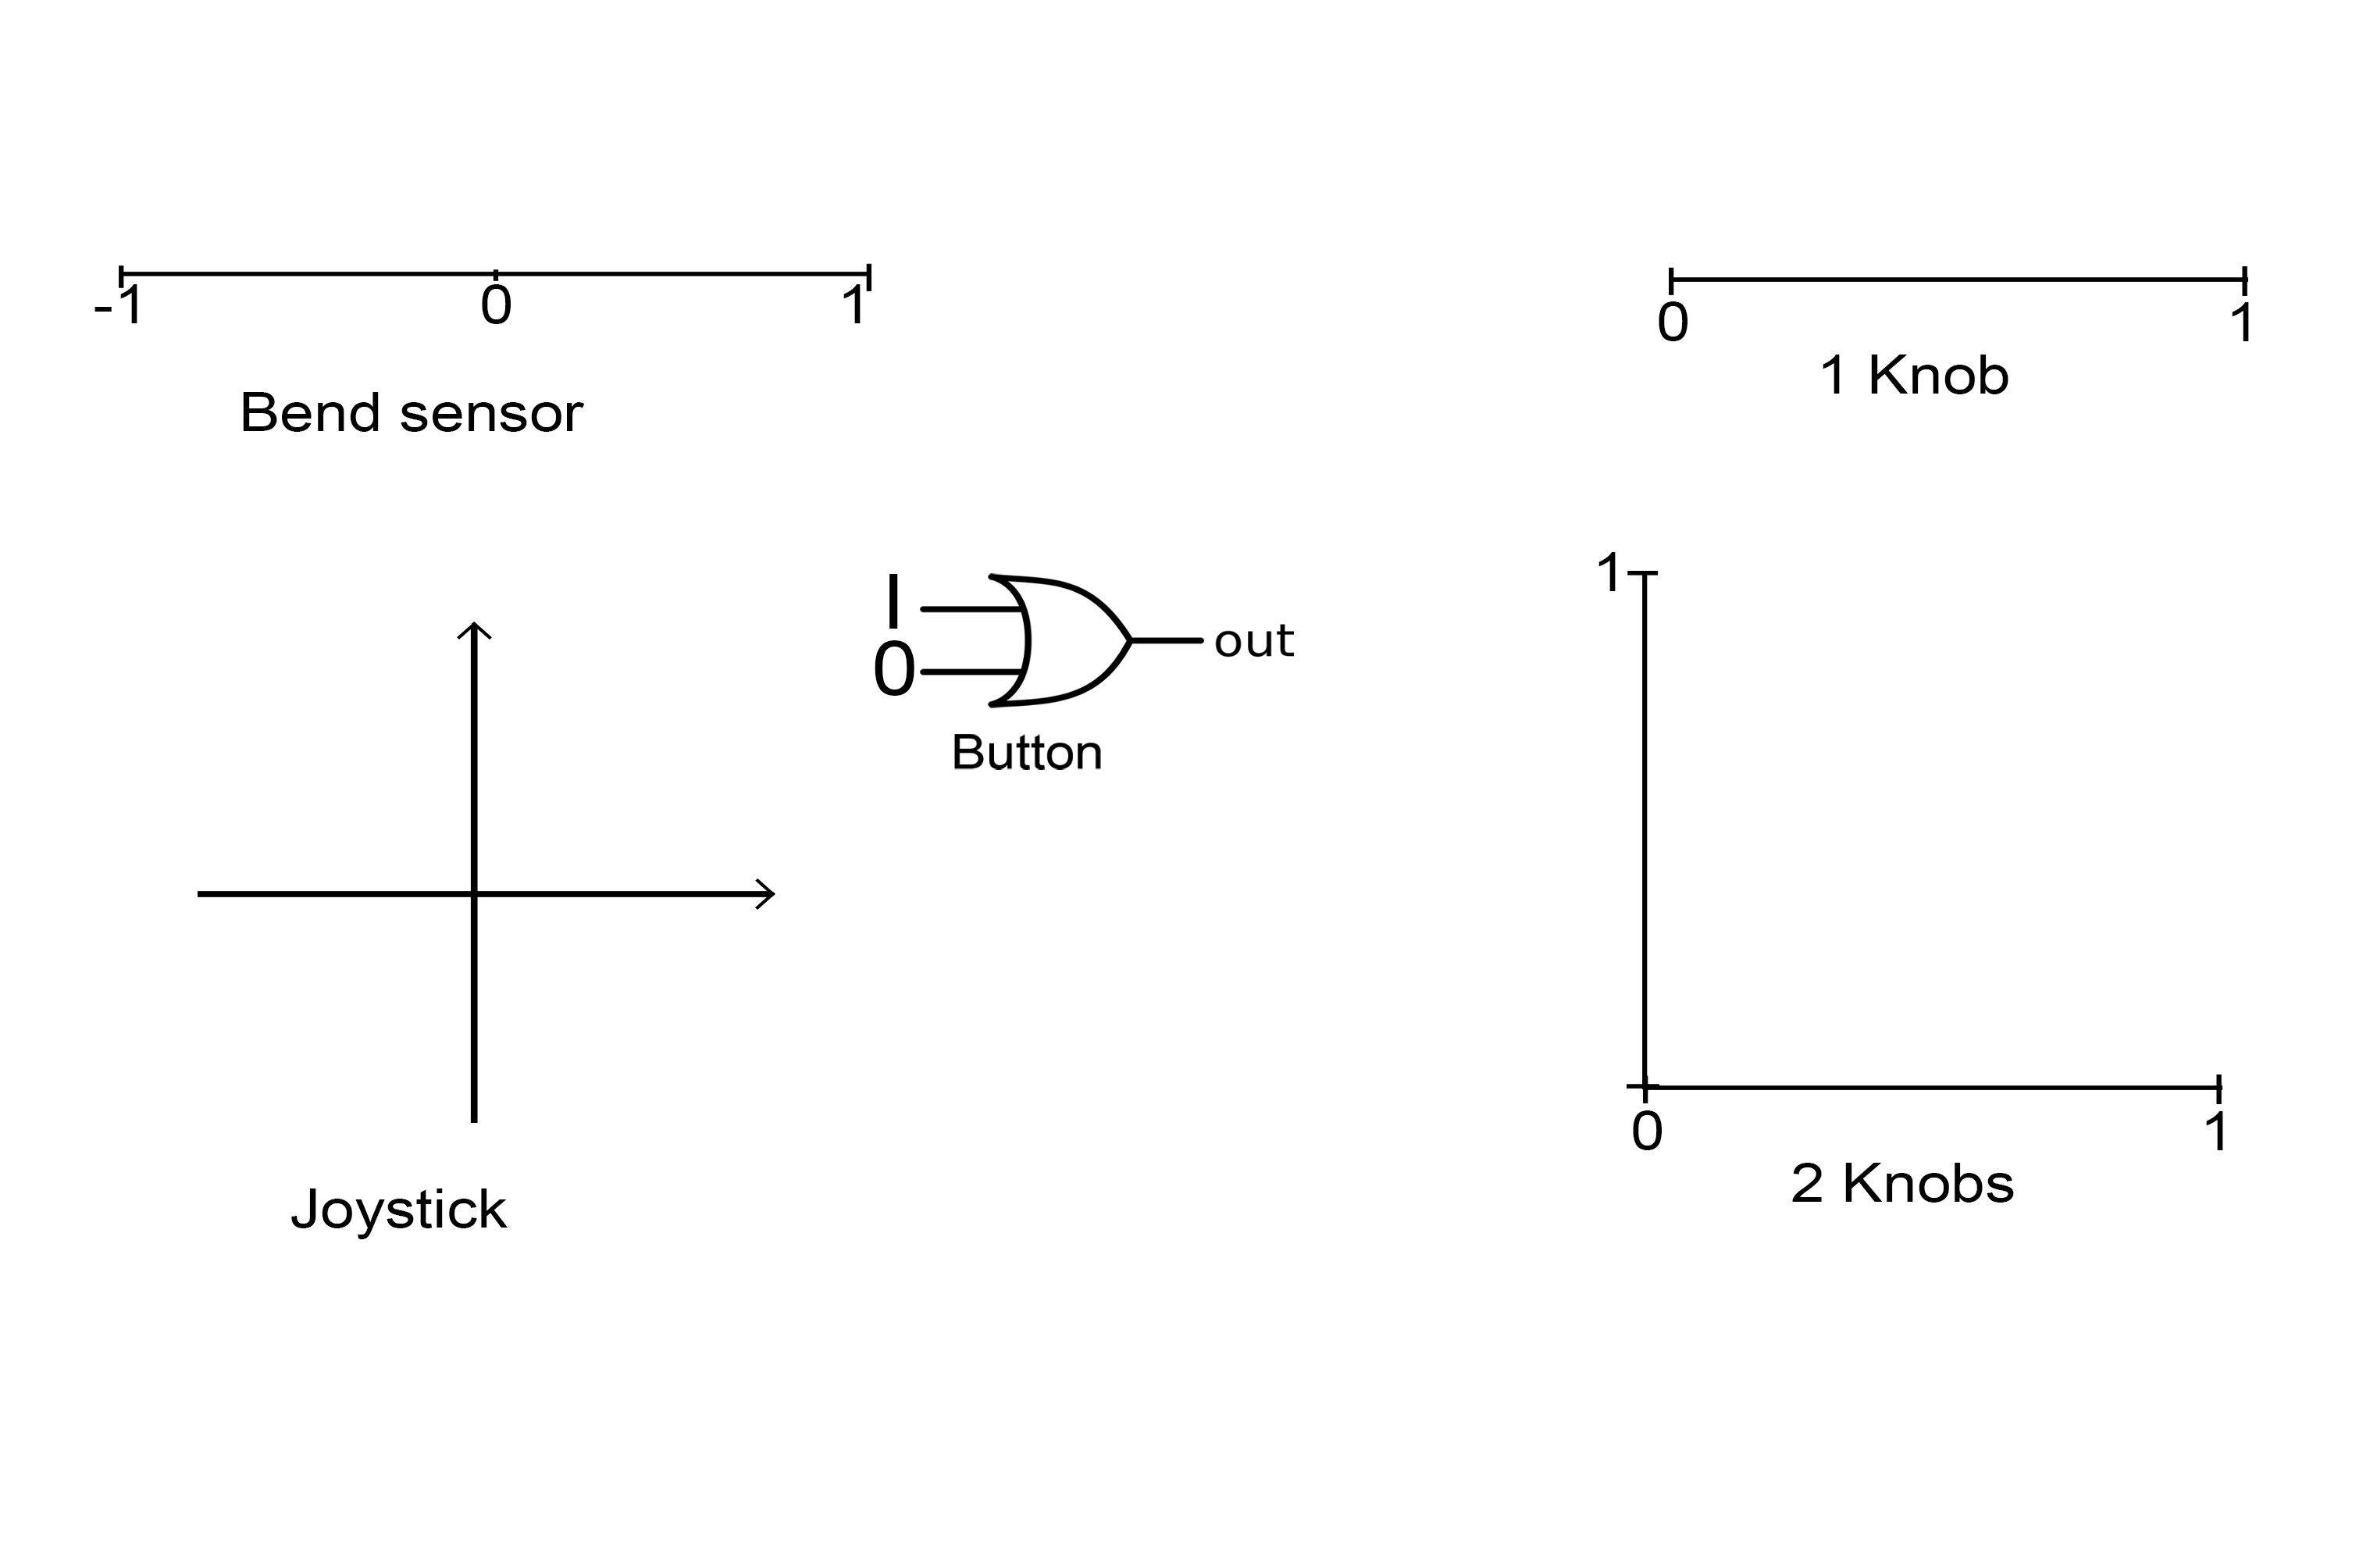
\includegraphics[width=1\textwidth]{Axis}
\caption{\label{fig:axis}}
\end{figure}


\todo{talk about what is the preference of different interfaces for the user (after test)}

Each of these peripheral devices makes the user interact with the prototype differently and changes the function of each device.

Figure \ref{fig:axis} shows the scales of which the different devices operate on, and how many different axis they are able to manipulate and to what length.
 
The joystick work by incorporating a variable on each axis, such that when the joystick is moved it alters the variables on the axis. 

There are multiple variable resistors to choose from. One of them being a knob the user can turn, which scales from 0 to 1 as well as a bend sensor that scales from negative 1 to positive 1. When the user alters the resistance in the system, the Arduino registers the change and send back a signal to the software in order to change the effect.

The way that these devices would be used, are as variable controller for the effect itself. Depending on what device is chosen, the integration for the user will be different. This will be tested in the iterations of the prototype and discussed further to make sure that the interface is user-friendly and easy to understand. 

\todo{expand upon the advantages and disadvantages of the different categories of devices}

\section{Early sketches and testing}
While sketching ideas for the design, the group encountered the obstacle of not knowing which electrical components to use. Therefore component test was with the purpose of deciding which component is the most intuitive to use. 

The test used 9 different electrical components consisting of the following:
\begin{itemize}
\item Button
\item Pressure sensor
\item Ultra sonic distance sensor
\item Telegraph-like button
\item Potentiometer Big/Small?
\item x
\item x
\item Slider
\item Bend sensor
\end{itemize}

These components were all mounted on a cardboard plate as seen on the figure below.

!!insert figure of pap thing og beskriv det!!

The test was conducted on 10 participants, all fellow students from Medialogy. The participants were explain by test facilitator 1 how each component worked and how to interact with them. They were told that they had to use all of the components one at a time in a numeral order and think out loud when using the components. Test facilitator 2 turned the volume of the music up and down, corresponding to how much the participant !!turned/clicked/slid/moved their hand!!.

Results showed that the participants preferred using the slider, showed on the figure below, when changing the volume of the music. New design sketches were created based on this result.







